
\section{UCM}

Per questa fase si è deciso di iniziare l’analisi con un modello semplice: conoscendo già i tipi di stagionalità, ne sono state aggiunte una giornaliera dummy e una settimanale sinusoidale, mentre per il level sono stati diversi tipi (random walk, local linear trend, ecc), per determinare il più adatto. 

Individuato il random walk with drift, si è poi passati a verificare se modellare le stagionalità in quel modo fosse effettivamente ottimale. Infatti, si è capito come il modo migliore fosse vederle entrambe scritte come sinusoidi. In particolare, dopo una serie di test, il numero ottimale di sinusoidi è di 5 e 3, rispettivamente per stagionalità stocastica giornaliera e settimanale. È importante notare che, al fine di evitare che l'algoritmo non raggiunga la convergenza, è stata impostata la varianza iniziale del modello ad un valore più consono, cioè la varianza della serie storica di training. 

L'aggiunta della componente di ciclo stocastico non ha portato miglioramenti al modello. Lo stesso vale per l'aggiunta dei regressori esterni dummy sulle festività, così come accadeva anche in ARIMA. 

Quindi, il modello che ottiene le migliori performance, in temini di AIC e MAPE (compromesso tra i due), è quello composto da:
\begin{itemize}
    \item random walk con drift
    \item 6 sinusoidi stocastiche per modellare la stagionalità giornaliera
    \item 2 sinusoidi stocastiche per modellare la stagionalità settimanale
\end{itemize}

Questo modello ottiene un AIC di -19414 e un MAPE di 11.13\%. Si notano, anche graficamente, le minori performance rispetto alla previsione ARIMA. 

\begin{figure}[H]
\centering
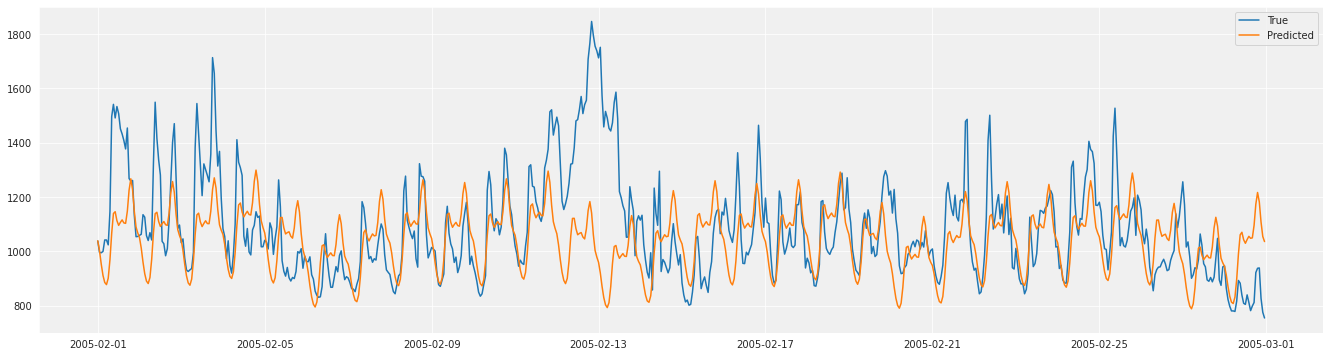
\includegraphics[width=14cm]{Pictures/prediction_ucm.png}
\caption{Previsione finale del modello UCM.}
\end{figure}

I residui del modello finale sono simili a quelli di ARIMA, mantenendo purtroppo ancora più memoria e correlazione. 

\begin{figure}[H]
\centering
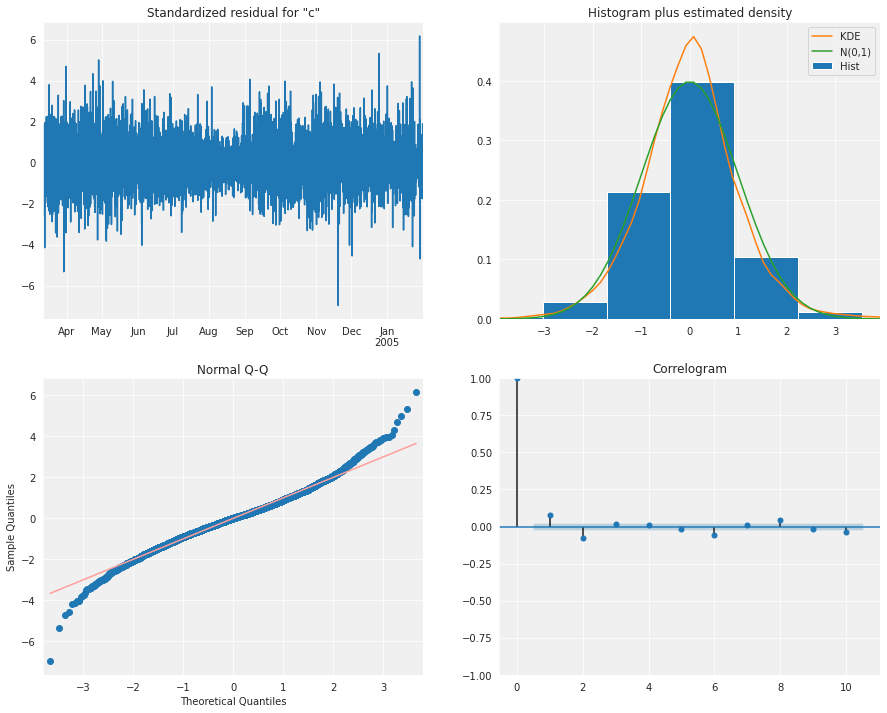
\includegraphics[width=12cm]{Pictures/summary_ucm.png}
\caption{Riepilogo sui residui del modello.}
\end{figure}


\vspace{0.5cm}